\documentclass[urlcolor=blue,dvipsnames]{beamer}

\usepackage[utf8]{inputenc}
\usepackage{fancybox,fancyvrb}
\usepackage{environ,xspace,empheq}

\usepackage{tikz}
\usetikzlibrary{arrows.meta,decorations.markings,decorations.pathreplacing,fadings,positioning}

\hypersetup{colorlinks,linkcolor=,urlcolor=cyan}

\beamertemplatenavigationsymbolsempty
\setbeamertemplate{footline}[frame number]
\usetheme{Pittsburgh}

%\makeatletter
%\newcommand{\tinytiny}{\@setfontsize{\tinytiny}{4pt}{4pt}}
%\makeatother

\newcommand\enumnum[1]{{\renewcommand{\insertenumlabel}{#1}%
      \usebeamertemplate{enumerate item} \,}}

\newcommand{\grad}{\nabla}
\newcommand{\ih}{\boldsymbol{\hat{\textbf{\i}}}}
\newcommand{\jh}{\boldsymbol{\hat{\textbf{\j}}}}
\newcommand{\vF}{\boldsymbol{\vec{\textbf{F}}}}
\newcommand{\Matlab}{\textsc{Matlab}\xspace}
\newcommand{\Octave}{\textsc{Octave}\xspace}


\title{7.4 Laplace Transforms: \\ convolutions only}

\subtitle{a lesson for MATH F302 Differential Equations}

\author{Ed Bueler, Dept.~of Mathematics and Statistics, UAF}

\date{\tiny \today}


\begin{document}
\setbeamertemplate{itemize item}{$\bullet$}
\setbeamertemplate{itemize subitem}{$\circ$}
\renewcommand{\thefootnote}{{\color{green} \arabic{footnote}}}

\begin{frame}
\titlepage

\centerline{\tiny for textbook: \, D. Zill, \emph{A First Course in Differential Equations with Modeling Applications}, 11th ed.}
%\color{green!40!blue}
\end{frame}

\newcommand{\LL}[1]{\mathcal{L}\left\{#1\right\}}
\newcommand{\LLi}[1]{\mathcal{L}^{-1}\left\{#1\right\}}



\begin{frame}{remember we have a decent table}

\vspace{-5mm}
\begin{center}
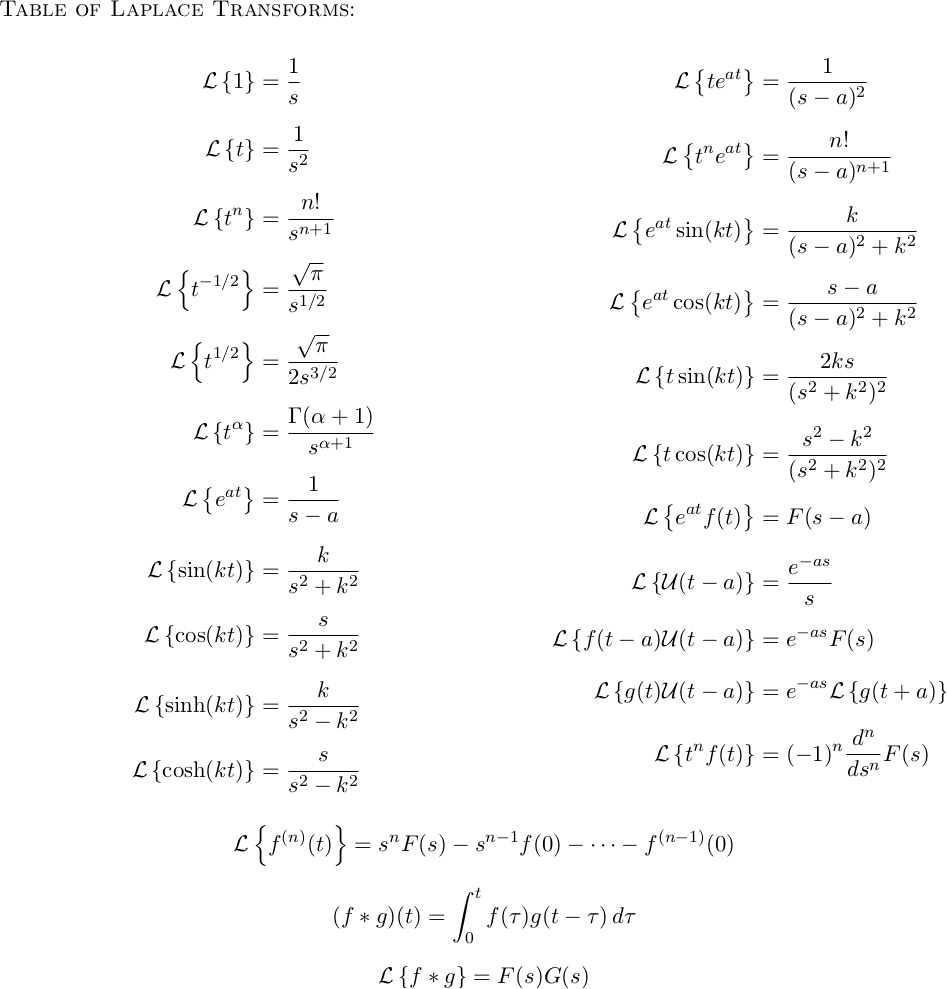
\includegraphics[height=80mm]{figs/fulllaplacetable}
\end{center}

\vspace{-13mm}
\alert{\emph{note last two entries $\to$}}
\end{frame}


\begin{frame}{convolution}

\begin{itemize}
\item the last two entries say:
\begin{align*}
(f \ast g)(t) &= \int_0^t f(\tau) g(t-\tau)\,d\tau \\
\LL{f \ast g} &= F(s) G(s)
\end{align*}
\end{itemize}
\end{frame}


\begin{frame}{X}

\begin{itemize}
\item X
\end{itemize}
\end{frame}


\begin{frame}{X}

\begin{itemize}
\item X
\end{itemize}
\end{frame}


\begin{frame}{like \S7.4 \#19}

\begin{itemize}
\item \emph{exercise 1.}  
\end{itemize}
\end{frame}


\begin{frame}{like \S7.4 \#26 and \#28}

\begin{itemize}
\item \emph{exercise 2.}  
\item \emph{exercise 3.}  
\end{itemize}
\end{frame}


\begin{frame}{like \S7.4 \#35}

\begin{itemize}
\item the convolution of $f(t)$ with the constant 1 is just an integral:
    $$f(t) \ast 1 = \int_0^t f(\tau) 1\,d\tau = \int_0^t f(\tau)\,d\tau$$
\item so
    $$\frac{F(s)}{s} = \LL{f(t)\ast 1}=\LL{\int_0^t f(\tau)\,d\tau}$$
\item \emph{exercise 4.}  use this to find the inverse Laplace transform:
    $$\LLi{\frac{1}{s(s-1)}} = \hspace{80mm}$$

\vspace{20mm}
\end{itemize}
\end{frame}


\begin{frame}{X}

\begin{itemize}
\item X
\end{itemize}
\end{frame}


\begin{frame}{expectations}

\begin{itemize}
\item just watching this video is \emph{not} enough!
     \begin{itemize}
     \item see ``found online'' videos and stuff at

     \centerline{\href{https://bueler.github.io/math302/week11.html}{\tt \color{cyan} bueler.github.io/math302/week11.html}}
     \item \emph{read} ``7.4.2 Transforms of Integrals'' in \S7.4
     \item \emph{do} the WebAssign exercises for section 7.4
     \end{itemize}
\end{itemize}
\end{frame}

\end{document}

